\documentclass[a4paper,10pt]{beamer}
\mode<presentation> {
\usetheme{Warsaw}
\setbeamercolor{structure}{fg=black!50!cyan}

% \setbeamercolor{structure}{fg=black!50!red}
}
\beamertemplatenavigationsymbolsempty
\usepackage{dsfont}
\usepackage{bm} 
\usepackage[english]{minitoc}
\usepackage{tcolorbox}
% \setcounter{minitocdepth}{2}
\usepackage[english]{babel}
% \usepackage{MnSymbol,wasysym}
\usepackage{tikzsymbols}
\usepackage{caption}
\usepackage{multicol}
\usepackage{bibentry}
\usepackage{varwidth}
  \usepackage{multirow,makecell,array}
  \usepackage{colortbl}
\usepackage[T1]{fontenc}
%\usepackage[latin1]{inputenc} 
\usepackage[utf8]{inputenc}
\usepackage{amsmath,amsfonts,amssymb,mathabx}
 \usepackage{mathrsfs}
\usepackage{graphicx}
   \usepackage{placeins}
\usepackage{hyperref}
\usepackage{algorithmicx}
\usepackage{algorithm}
\usepackage{algpseudocode}
\usepackage{changepage}
\usepackage{slantsc}
\setcounter{tocdepth}{1}
\usepackage{pifont}
\usepackage{wasysym}
\newcommand{\cmark}{\ding{51}}%
\newcommand{\xmark}{\ding{55}}%
\useinnertheme{circles}
\usefonttheme[onlymath]{serif}

 \setlength{\fboxrule}{1pt}
%Change frame margins
% \newcommand\Wider[2][3em]{%
% \makebox[\linewidth][c]{%
%   \begin{minipage}{\dimexpr\textwidth+#1\relax}
%   \raggedright#2
%   \end{minipage}%
%   }%
% }

\usepackage{tikz}
\usetikzlibrary{decorations.pathreplacing,calc}
\newcommand{\tikzmark}[1]{\tikz[overlay,remember picture] \node (#1) {};}

\newcommand*{\AddNote}[4]{%
    \begin{tikzpicture}[overlay, remember picture]
        \draw [decoration={brace,amplitude=0.5em},decorate,ultra thick,red]
            ($(#3)!(#1.north)!($(#3)-(0,1)$)$) --  
            ($(#3)!(#2.south)!($(#3)-(0,1)$)$)
                node [align=center, text width=1.6cm, pos=0.5, anchor=west] {#4};
    \end{tikzpicture}
}%

\renewcommand{\pgfuseimage}[1]{\includegraphics[scale=.75]{#1}}

%Define colors
\definecolor{white}{rgb}{1,1,1}
\newcommand\white[1]{\textcolor{white} {#1} }
\definecolor{gray}{rgb}{.91, .91, .91}

\definecolor{green}{rgb}{0,0.45,0}
\newcommand\gr[1]{\textcolor{green} {#1} }

  \newcommand\bk[1]{\textcolor{black} {#1} }
  
  \newcommand\red[1]{\textcolor{red} {#1} }
  
  \newcommand\bl[1]{\textcolor{blue} {#1} }
  
  \newcommand\black[1]{\textcolor{black} {#1} }
  
\definecolor{royalmagenta}{rgb}{.79,.17,.57}
  \newcommand\ma[1]{\textcolor{royalmagenta} {#1} }

    
\definecolor{magenta}{rgb}{1,0,1}
  \newcommand\magenta[1]{\textcolor{magenta} {#1} }
  
\definecolor{salmonpink}{rgb}{1,.6,.6}
  \newcommand\sapi[1]{\textcolor{salmonpink} {#1} }
  
\definecolor{cyan}{rgb}{0,0.6,1}
  \newcommand\cy[1]{\textcolor{cyan} {#1} }
  
\definecolor{yellow}{rgb}{1,0.85,0}
  \newcommand\yellow[1]{\textcolor{yellow} {#1} }
  
\definecolor{regalia}{rgb}{0.52, 0.18, 0.6}
\newcommand\vio[1]{\textcolor{regalia}{#1}}

\definecolor{orange}{rgb}{1, 0.55, 0}
\newcommand\ora[1]{\textcolor{orange}{#1}}

\newtheorem{proposition}{Proposition}

%Insert frame numbers

\title[A RBM for variational inequalities]
{Reduced basis for variational inequalities Application to contact mechanics}
\author[Amina Benaceur]{
\underline{\rmfamily\textsc{Amina Benaceur}}, {\rmfamily\textsc{A. Ern}}
and {\rmfamily\textsc{V. Ehrlacher}}
}
\institute{
{\color{white}me} \\

}

\date{March $12^{th}$, $2025$}


\titlegraphic{\vspace{-1cm}
\begin{adjustwidth}{-0.2cm}{0cm}
%\includegraphics[width=1.2cm]{edf.png}
\hspace*{3.7cm}~%
%\includegraphics[width=1.2cm]{mit.png}
\hspace*{3.1cm}~%
 %  \includegraphics[width=1.2cm]{enpc.png}\vspace{0.2cm}
   \end{adjustwidth}
}
\begin{document}
\begin{frame}%
\vfill
\vfill
\vfill
\titlepage
\end{frame}
% \setbeamertemplate{footline}[frame number]{}
 \expandafter\def\expandafter\insertshorttitle\expandafter{%
 \insertshorttitle\hfill
  \insertframenumber/29}
\subsection{Industrial context}


\begin{frame}
\addtocounter{framenumber}{-1}
\begin{columns}
\hspace{0.5cm}
\begin{column}{9cm}
{\bfseries Motivations for contact}
\begin{itemize}
 \item Long-standing question in many contexts...
 \item Present industrial context
  \begin{itemize} 
\item Behavior of valve components
\item Costly simulations ($\approx$ 12h using `\texttt{code\_aster}')
\end{itemize}
\item \bl{Nonlinearities, constraints}
\end{itemize}
\medskip

{\bfseries Challenge}
\begin{itemize} 
\item Expensive for parameterized studies
\end{itemize}
\medskip

{\bfseries Goal}
\begin{itemize} 
    \item Nonlinearly constrained model reduction
\end{itemize}
\end{column}
\hspace{-1.2cm}
\begin{column}{5cm}
\vspace{-0.5cm}
\begin{figure}[h!]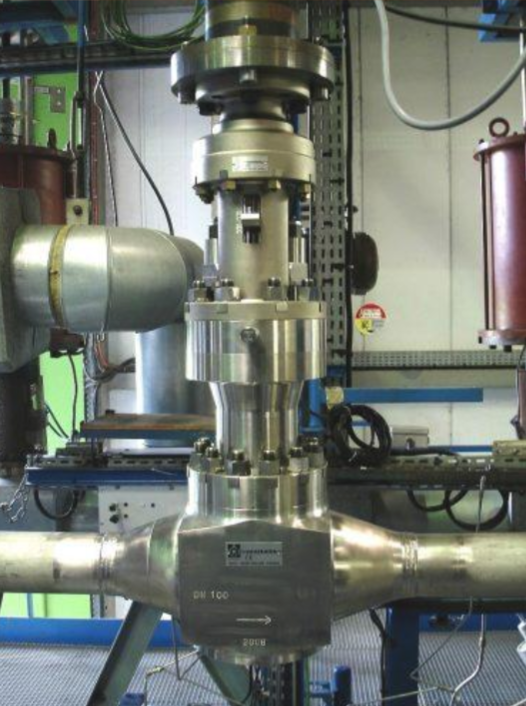
\includegraphics[width=0.6\textwidth]{./images/real_valve.png} 
\captionsetup{justification=centering,margin=0cm}
\centering 
\end{figure}
\vspace{-0.3cm}
\begin{figure}[h!]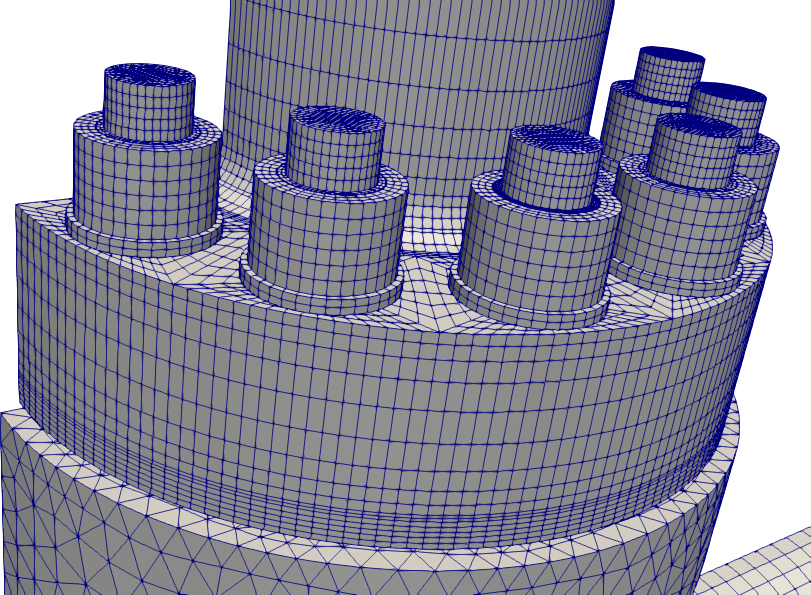
\includegraphics[width=0.6\textwidth]{./images/intro_contact.png} 
\captionsetup{justification=centering,margin=0cm}
\centering 
\end{figure}
\end{column}
\end{columns}
\end{frame}


\subsection{Variational inequalities with linear constraints}
\begin{frame}
\frametitle{Variational inequalities with linear constraints}
{\bfseries Reduced basis procedures}
\medskip

\mbox{
\begin{minipage}{\textwidth}
\begin{thebibliography}{1}
\item {\footnotesize\bl{\textit{Haasdonk, Salomon, Wohlmuth.}}A reduced basis method for parametrized variational inequalities. \bl{2012.}}
\item {\footnotesize\bl{\textit{Balajewicz, Amsallem, Farhat.}}Projection-based model reduction for contact
problems. \bl{2016.}} 
\item {\footnotesize\bl{\textit{Fauque, Ramiere, Ryckelynck.}}Hybrid hyper-reduced modeling for contact mechanics problems. \bl{2018.}}
\end{thebibliography}
\end{minipage}
}
\bigskip

{\bfseries Related work}
\medskip

\mbox{
\begin{minipage}{\textwidth}
\begin{thebibliography}{1}
\item {\footnotesize\bl{\textit{Burkovska, Haasdonk, Salomon, Wohlmuth.}}Reduced basis methods for pricing
options with the Black--Scholes and Heston models. \bl{ 2014.}}
\item {\footnotesize\bl{\textit{Glas, Urban.}}Numerical investigations of an error bound for reduced basis approximations of non-coercive variational inequalities. \bl{ 2015.}}
\item {\footnotesize\bl{\textit{Bader, Zhang, Veroy.}}An empirical interpolation approach to reduced basis approximations for variational inequalities, \bl{2016.}}
\item {\footnotesize\bl{\textit{Burkovska.}}PhD thesis. \bl{ 2016.}}
\end{thebibliography}
\end{minipage}
}

\end{frame}

\begingroup
\setbeamertemplate{footline}{}
\begin{frame}[noframenumbering]
\frametitle{Outline}
\tableofcontents
\end{frame}
\endgroup
%---------------------
%---------------------

\section{Elastic contact problem}
\subsection{Elastic equation}
\begin{frame}\frametitle{Elastic contact problem}
% Linearized 
Strain tensor
% \vspace{-0.3cm}
$$
 \varepsilon(v): = \frac{1}{2}(\nabla v + \nabla v^T)
$$
Stress tensor
% \vspace{-0.3cm}
$$
\sigma(v) = \frac{E\nu}{(1+\nu)(1+2\nu)} {\rm tr}(\varepsilon(v))\mathcal I+\frac{E}{(1+\nu)}\varepsilon(v)
$$
\begin{center}
$E$: Young modulus
\qquad
$\nu$: Poisson coefficient
\smallskip 

\begin{tcolorbox}[colback=blue!5,colframe=black!50!cyan,width = .7\linewidth,title={Parametric equilibrium condition}, halign = center]
$\nabla\cdot\sigma(u(\mu)) = \ell(\mu) \quad \text{in } \red{\Omega(\mu)}
$
\end{tcolorbox}
\end{center}
$$ a(\mu;v,w) = \int_{\red{\Omega(\mu)}}\sigma(v):\varepsilon(w)
\quad\text{and}\quad
 f(\mu;w) = \int_{\red{\Omega(\mu)}}\ell(\mu)w
$$
Other nonlinearities can be handled
\end{frame}


\subsection{Non-interpenetration condition}
\begin{frame}\frametitle{Non-interpenetration condition}
\vspace{-.3cm}
\begin{center}
 {\bfseries \hspace{.7cm} Initial configuration \hspace{1.cm} Deformed configuration}
\end{center}
\vspace{-.2cm}\begin{figure}
\qquad
 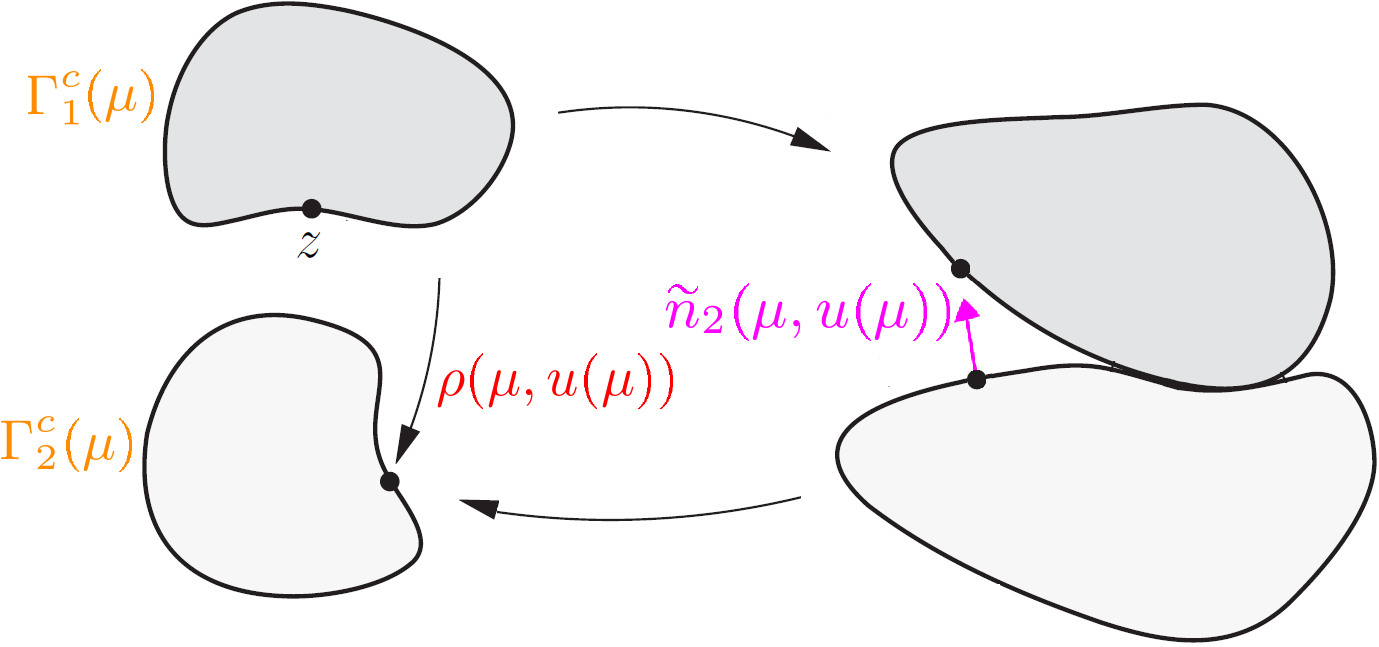
\includegraphics[width=.7\textwidth]{./images/contact/scheme.png}
 \centering
\end{figure}
\vspace{0.1cm}

\pause
Consider $\mathcal V(\mu)=H^1(\Omega_1(\mu)) \times H^1(\Omega_2(\mu))$

Admissible solutions are denoted $u(\mu)=(u_1(\mu),u_2(\mu))\in\mathcal V(\mu)$

\hspace{-1.7cm}
% \fbox{
\begin{minipage}{1.2\textwidth}
\small{
For all $z \in \ora{\Gamma^c_1(\mu)}$
\vspace{-0.3cm}
$$
\hspace{-2.1cm}\underbrace{\left(\gr{u_1(\mu)}(z)- \left(\gr{u_2(\mu)}\circ\red{\rho(\mu,\bl{u(\mu)})}\right)(z)\right)}_{\rm displacement\ difference}\cdot 
\magenta{\widetilde n_2(\mu,\bl{u(\mu)})}(z)
\geq
\underbrace{\big(\red{\rho(\mu,\bl{u(\mu)})}(z)-z\big)}_{\rm initial\ gap}\cdot \magenta{\widetilde n_2(\mu,\bl{u(\mu)})}(z)
$$
}
\vspace{-0.3cm}

{\small $\implies$ Proof : \bl{Benaceur,}PhD thesis}
\end{minipage}
\end{frame}

\begin{frame}\frametitle{Non-interpenetration condition}
\only<1>
\addtocounter{framenumber}{-1}
\vspace{-.3cm}
\begin{center}
 {\bfseries \hspace{.7cm} Initial configuration \hspace{1.cm} Deformed configuration}
\end{center}
\vspace{-.2cm}\begin{figure}
\qquad
 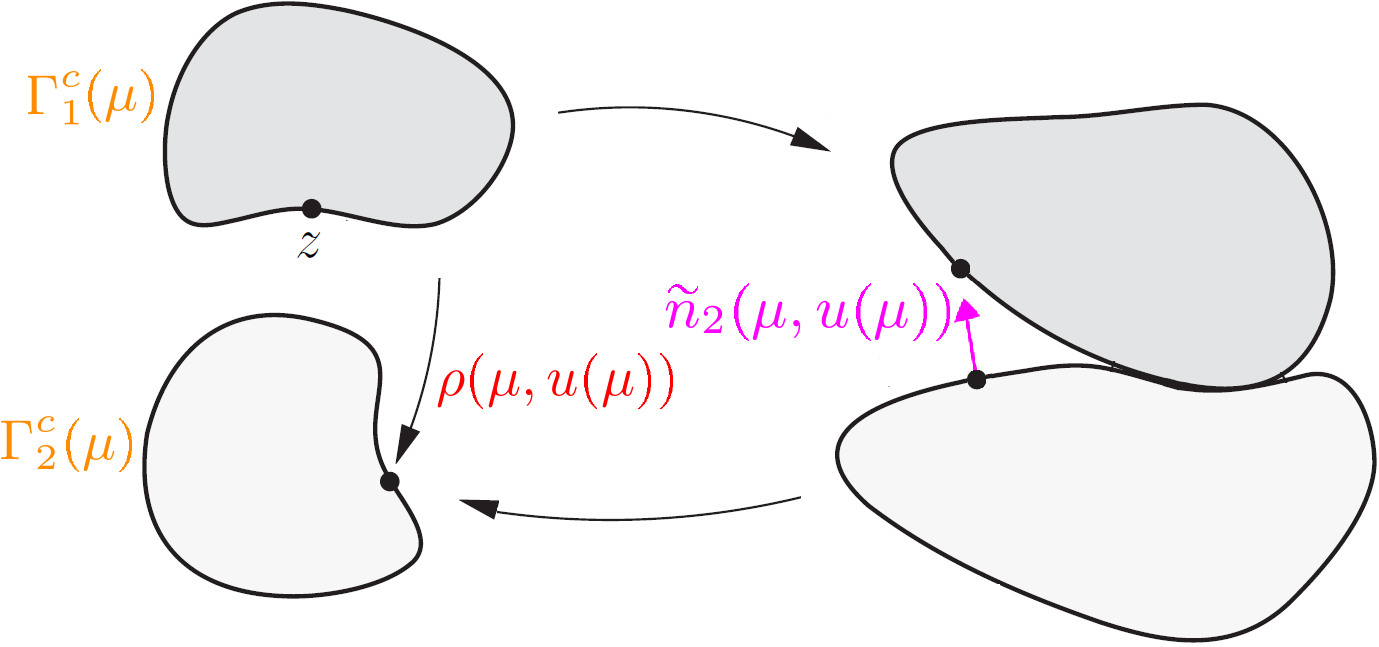
\includegraphics[width=.7\textwidth]{./images/contact/scheme.png}
 \centering
\end{figure}
\vspace{0.1cm}

Consider $\mathcal V(\mu)=H^1(\Omega_1(\mu)) \times H^1(\Omega_2(\mu))$

Admissible solutions are denoted $u(\mu)=(u_1(\mu),u_2(\mu))\in\mathcal V(\mu)$

\hspace{-1.7cm}
% \fbox{
\begin{minipage}{1.2\textwidth}
\small{
For all $z \in \ora{\Gamma^c_1(\mu)}$
\vspace{-0.3cm}
$$
\hspace{-2.1cm}\underbrace{\left(\gr{u_1(\mu)}(z)- \left(\gr{u_2(\mu)}\circ\red{\rho(\mu,\bl{u(\mu)})}\right)(z)\right)\cdot 
\magenta{\widetilde n_2(\mu,\bl{u(\mu)})}(z)}_{-k(\mu,\bl{u(\mu)};\gr{u(\mu)})}
\geq
\underbrace{\big(\red{\rho(\mu,\bl{u(\mu)})}(z)-z\big)\cdot \magenta{\widetilde n_2(\mu,\bl{u(\mu)})}(z)}_{-g(\mu,\bl{u(\mu)})}
$$
}
\vspace{-0.3cm}

{\small $\implies$ Proof: \bl{Benaceur,}PhD thesis}
\end{minipage}
\end{frame}

\section{Abstract model problem}

\subsection{Abstract model problem}
\begin{frame}\frametitle{Model problem}
% \addtocounter{framenumber}{-1}
$\Omega(\mu)$ : bounded domain in $ \mathbb{R}^d$ with a contact boundary $\Gamma^c_1(\mu)\subset\partial\Omega(\mu)$

$\mathcal V(\mu)$ : Hilbert space on $\Omega(\mu)$

$\mathcal P$: parameter set

\medskip

For many values $\mu\in\mathcal P$: 
Find $u(\mu)\in\mathcal V$ such that
\begin{center}
\begin{tcolorbox}[colback=blue!5,colframe=black!50!cyan,width = .7\linewidth,halign = center]
$
\begin{alignedat}{2}
& u(\mu)=\underset{v \in \mathcal V(\mu)}{\mathrm{argmin}}\ \frac{1}{2}a(\mu;v,v)- f(\mu;v) \\
& k(\mu,\bl{u(\mu)};\gr{u(\mu)})\leq g(\mu,\bl{u(\mu)})\quad \text{a.e. on }\Gamma^c_1(\mu)
 \end{alignedat}
$
\end{tcolorbox}
\end{center}
$k(\mu,\cdot;\cdot)$ is semi-linear : natural for contact problems\\
\hspace{3.45cm} handy for iterative solution methods

% For model reduction, $\Omega$ will be considered \bl{parametric ($\Omega(\mu)$)}
\end{frame}


\subsection{Lagrangian formulation}
\begin{frame}\frametitle{Lagrangian formulation}
We consider 
\begin{itemize}
 \item the convex cone $\ma{\mathcal W(\mu)}:=L^2(\Gamma^c_1(\mu),\mathbb R_+)$
\item the Lagrangian $\mathcal L(\mu):\bl{\mathcal V(\mu)}\times\ma{\mathcal W(\mu)}\rightarrow \mathbb R$ defined as
 \vspace{-0.2cm}
 
\hspace{-0.9cm}
 \begin{minipage}{1.\textwidth}
\[\boxed{
$$
 \mathcal L(\mu)(\bl{v},\ma{\eta}):=\frac{1}{2}a(\mu;\bl{v},\bl{v})- f(\mu;\bl{v})
 +\left(\int_{\Gamma_1^c(\mu)}k(\mu,\bl{v};\bl{v})\ma{\eta}- \int_{\Gamma_1^c(\mu)}g(\mu,\bl{v})\ma{\eta}\right)
 $$
 }\]
\end{minipage}
\end{itemize}

 \bigskip
 
Find $(\bl{u(\mu)},\ma{\lambda(\mu)})\in \bl{\mathcal V(\mu)}\times\ma{\mathcal W(\mu)}$ such that 
\begin{center}
\begin{tcolorbox}[colback=blue!5,colframe=black!50!cyan,width = .7\linewidth]
$ (\bl{u(\mu)},\ma{\lambda(\mu)})={\rm arg}\ \underset{\bl{v \in \mathcal V(\mu)}, \ma{\eta \in \mathcal W(\mu)}}{\rm minmax}\ \mathcal L(\mu)(\bl{v},\ma{\eta})$
\end{tcolorbox}
\end{center}

\bl{$u(\mu)$}is the primal solution, 
\ma{$\lambda(\mu)$}is the dual solution
\end{frame}

\subsection{Discrete FEM formulation}
\begin{frame}\frametitle{Discrete FEM formulation}
\vspace{-.2cm}
\begin{enumerate}
 \item FEM space ($\mathcal N\gg1$)
\vspace{-.3cm}
$$\bl{V_{\mathcal N}(\mu):={\rm span}\{\phi_1(\mu),\ldots,\phi_{\mathcal N}(\mu)\} \subset \mathcal V(\mu)}$$
\item FEM convex cone ($\mathcal R\gg1$)
\vspace{-.3cm}
$$\ma{W_{\mathcal R}(\mu):=\red{{\rm span}_+}\{\psi_1(\mu),\ldots,\psi_{\mathcal R}(\mu)\} \subset \mathcal W(\mu)}$$
\end{enumerate}
\pause

\begin{center}
\begin{tcolorbox}[colback=blue!5,colframe=black!50!cyan,width = .9\linewidth,title={Algebraic FEM formulation}, halign = center, halign title = flush center]
\vspace{-.4cm}
 \begin{align*}\label{eq:lag_fem_disc}
(\bl{\mathbf u(\mu)}, \ma{{\bm\lambda}(\mu)})={\mathrm{arg}}\ \underset{\bl{\mathbf v \in \mathbb R^{\mathcal N},}
 \ma{{\bm \eta} \in \mathbb R_+^{\mathcal R}}}{\mathrm{minmax}} \
 &\Big\{\frac{1}{2}\bl{\mathbf v^T} \mathbf A(\mu) \bl{\mathbf v}- \bl{\mathbf v^T}\mathbf f(\mu)\\
&+\ma{{\bm \eta}^T} \big(\mathbf K(\mu,\bl{\mathbf v})\bl{\mathbf v}- \mathbf g(\mu,\bl{\mathbf v})\big)\Big\}
\end{align*}
\end{tcolorbox}
\end{center}
$$
\begin{alignedat}{2}
&\mathbf A(\mu)_{ij} = a(\mu;\bl{\phi_j(\mu)},\bl{\phi_i(\mu)})
 \qquad
% &&\mathbf f(\mu)_j = f(\mu;\bl{\phi_j(\mu)})
% \\
& \mathbf K(\mu,w)_{ij} = \int_{\Gamma^c_1(\mu)}k(\mu,w;\bl{\phi_{j}(\mu)})\ma{\psi_i(\mu)}
% \qquad
% &&\mathbf g(\mu,w)_{j} = \int_{\Gamma^c_1}g(\mu,w)\ma{\psi_j(\mu)}
 \end{alignedat}
$$
Additional nonlinearity caused by 
spatial dicretization
\end{frame}


\begin{frame}\frametitle{The Ka\v{c}anov method}
\begin{itemize}
 \item Iterative procedure
\item Consists in solving the following problems : For all $k\geq 1$
\end{itemize}
\begin{center}
\begin{tcolorbox}[colback=blue!5,colframe=black!50!cyan,width =1.05\linewidth]
\vspace{-.4cm}
$$
\hspace{-.5cm}
\begin{alignedat}{2}
(\bl{\mathbf u^k(\mu)}, \ma{{\bm\lambda}^k(\mu)})=
{\rm arg}\ \underset{\substack{\mathbf v \in \mathbb R^{\mathcal N}, \mathbf \eta \in \mathbb R_+^{\mathcal R}}}{\rm min max}\ 
&\frac{1}{2}\mathbf v^T \mathbf A(\mu) \mathbf v- \mathbf v^T\mathbf f(\mu) \\
&+ {\bm \eta}^T \big(\mathbf K(\mu,\bl{\mathbf u^{\red{k-1}}(\mu)})\mathbf v - \mathbf g(\mu,\ma{{\bm \lambda}^{\red{k-1}}(\mu)})\big)
\end{alignedat}
$$
\end{tcolorbox}
\end{center}
\begin{itemize}
 \item Stopping criteria
\end{itemize}
$$
 \frac{\|\mathbf u^k(\mu)-\mathbf u^{k-1}(\mu)\|_{\mathbb R^{\mathcal N}}}{\|\mathbf u^{k-1}(\mu)\|_{\mathbb R^{\mathcal N}}}\leq\epsilon_{\rm ka}^{\rm pr}
 \qquad
 \frac{\|\mathbf {\bm \lambda}^k(\mu)-\mathbf  {\bm \lambda}^{k-1}(\mu)\|_{\mathbb R^{\mathcal N}}}{\|\mathbf  {\bm \lambda}^{k-1}(\mu)\|_{\mathbb R^{\mathcal N}}}\leq\epsilon_{\rm ka}^{\rm du}
$$
\end{frame}

\section{The reduced-basis model}
\subsection{Reference configuration}
\begin{frame}\frametitle{The reduced-basis model: Reference configuration}
Geometric mapping $h(\mu)$ defined on a reference domain $\widecheck{\Omega}$ (with $I=2$)
\begin{center}
\begin{tcolorbox}[colback=blue!5,colframe=black!50!cyan,width = .5\linewidth]
\vspace{-.4cm}
$$
\begin{alignedat}{2}
\red{h(\mu)}:\ &\widecheck{\Omega}&&\rightarrow\red{\Omega(\mu)}\\
&\ x &&\mapsto \sum_{i=1}^I \red{h_i(\mu,x)}\mathbf 1_{\widecheck{\Omega}_i}(x)
\end{alignedat}
$$
\vspace{-.4cm}
\end{tcolorbox}
\end{center}
\pause
\vspace{-.1cm}
\begin{equation*}
\Omega_i(\mu) = h(\mu)(\widecheck{\Omega}_i)
\quad\forall i\in\{1,2\}
\end{equation*}
\begin{equation*}
\Gamma_i^c(\mu) = h(\mu)(\widecheck{\Gamma}^c_i)
\quad\forall i\in\{1,2\}
\end{equation*}\vspace{-.8cm}

\begin{columns}
 \begin{column}{.5\textwidth}
 \begin{center}
{\bfseries Reference Hilbert space}
 \end{center}
 $$\bl{\widecheck{\mathcal V}:=H^1(\widecheck\Omega;\mathbb R^d)}$$
 \begin{center}
{\bfseries Parametric Hilbert space}
 \end{center}
$$
 \bl{\mathcal V(\mu)}\bl{=\widecheck{\mathcal V}\circ h(\mu)^{-1}}
$$
 \end{column}
 \begin{column}{.5\textwidth}
 \begin{center}
{\bfseries Reference convex cone}
\end{center}
$$\ma{\widecheck{\mathcal W}:=L^2(\widecheck\Gamma_1^c;\mathbb R_+)}$$
 \begin{center}
{\bfseries Parametric convex cone}
 \end{center}
$$
\ma{\mathcal W(\mu)=\widecheck{\mathcal W}\circ h(\mu)^{-1}_{|\Gamma_1^c(\mu)}}
$$
 \end{column}
\end{columns}
% \bigskip
% 
% Parametric Hilbert space \qquad\qquad
% Parametric convex cone
% \begin{align*}
%  \bl{\mathcal V(\mu)}&\bl{=\widecheck{\mathcal V}\star h(\mu)^{-1}}
% \qquad\qquad\qquad\
%  &&\ma{\mathcal W(\mu)=\widecheck{\mathcal W}\star h^{-1}(\mu)_{|\Gamma_1^c(\mu)}}\\
%  &\bl{=\{\widecheck v\circ h(\mu)^{-1}\ |\ \widecheck v\in\widecheck{\mathcal V}\}}
%  \quad
%  &&\qquad\ \ \ma{=\{\widecheck\eta\circ h^{-1}(\mu)_{|\Gamma_1^c(\mu)}\ |\ \widecheck\eta\in\widecheck{\mathcal W} \}}
% \end{align*}
\end{frame}


\subsection{Reduced basis spaces}
\begin{frame}\frametitle{Reduced basis spaces}
\begin{columns}
 \begin{column}{.5\textwidth}
 \begin{center}
{\bfseries Primal RB subspace}
 \end{center}
\begin{equation*}\label{eq:ref_spaces}
 \quad\bl{\widecheck V_N\subset\widecheck V_{\mathcal N}\subset\widecheck{\mathcal V}}
\end{equation*}
$$\quad\bl{\widecheck V_{N} = {\rm span}\{\widecheck\theta_1,\ldots,\widecheck\theta_{N}\}}$$
 \end{column}
 \begin{column}{.5\textwidth}
 \begin{center}
{\bfseries Dual RB subcone}
 \end{center}
\begin{equation*}
 \ma{\widecheck W_{R}\subset\widecheck W_{\mathcal R}\subset\widecheck{\mathcal W}}
\end{equation*}
$$
\ma{\widecheck W_{R} = \red{{\rm span}_+}\{\widecheck\xi_1,\ldots,\widecheck\xi_{R}\}}$$
 \end{column}
\end{columns}
\bigskip
\pause

\begin{center}
{\bfseries RB approximations}
\end{center}
\vspace{-0.2cm}
\begin{equation*}
\quad\bl{\widehat{u}(\mu)=\sum_{n=1}^N \widehat{u}_n(\mu)\widecheck\theta_n\circ \red{h(\mu)^{-1}}}\qquad
\ma{\widehat{\lambda}(\mu)=\sum_{n=1}^{R} \widehat{\lambda}_n(\mu)\widecheck\xi_n\circ \red{h(\mu)^{-1}}}
\end{equation*}
\end{frame}

\subsection{Reduced problem}
\begin{frame}\frametitle{Reduced problem}
\vspace{-.6cm}
\begin{center}
\begin{tcolorbox}[colback=blue!5,colframe=black!50!cyan,width = .9\linewidth]
\vspace{-.4cm}
 \begin{align*}
(\bl{\widehat{\mathbf u}(\mu)}, \ma{{\bm {\widehat \lambda}(\mu)}})={\mathrm{arg}}\ 
\underset{\bl{\widehat{\mathbf v} \in \mathbb R^N},\ma{\bm{\widehat \eta} \in \mathbb R_+^{R}}}{\mathrm{minmax}}\ 
&\Big\{\frac{1}{2}\bl{\widehat{\mathbf v}^T} \widehat{\mathbf A}(\mu) \bl{\widehat{\mathbf v}}- \bl{\widehat{\mathbf v}^T}\widehat{\mathbf f}(\mu)\\
&+\ma{\bm{\widehat\eta}^T}\big( \widehat{\mathbf K}(\mu,\bl{\widehat{\mathbf v}})\bl{\widehat{\mathbf v}} - \widehat{\mathbf g}(\mu,\bl{\widehat{\mathbf v}})\big)\Big\}
\end{align*}
\end{tcolorbox}
\end{center}
$$\widehat{\mathbf A}(\mu)\in\mathbb R^{\bl{N\times N}}
\quad
\widehat{\mathbf f}(\mu)\in\mathbb R^{\bl N}
\quad
{\widehat{\mathbf K}}(\mu,\widehat{\mathbf v})\in\mathbb R^{{\ma{R}\times \bl{N}}}
\quad
\widehat{\mathbf g}(\mu,\widehat{\mathbf v})\in\mathbb R^{\ma R}$$
\pause
\vspace{-.4cm}
 \begin{subequations}
 \begin{align*}
&\widehat{\mathbf A}(\mu)_{pn} = a(\red{\mu};\widecheck\theta_n\circ\red{h(\mu)^{-1}},\widecheck\theta_p\circ \red{h(\mu)^{-1}})\\
% &\widehat{\mathbf f}(\mu)_p = f(\red{\mu};\widecheck\theta_p\circ\red{h(\mu)^{-1}})\\
&{\widehat{\mathbf K}}(\mu,\widehat{\mathbf v})_{pn} = \int_{\red{\Gamma^c_1(\mu)}}k\bigg(\red{\mu},\sum_{i=1}^N\widehat v_i\widecheck\theta_i\circ \red{h(\mu)^{-1}};\widecheck\theta_n\circ\red{h(\mu)^{-1}}\bigg)\widecheck\xi_p\circ \red{h(\mu)^{-1}}\\
%  &\widehat{\mathbf g}(\mu,\widehat{\mathbf v})_p = \int_{\red{\Gamma^c_1(\mu)}}g\left(\red{\mu},\sum_{i=1}^N\widehat v_i\widecheck\theta_i\circ \red{h(\mu)^{-1}}\right)\widecheck\xi_p\circ \red{h(\mu)^{-1}}
 \end{align*}
\end{subequations}
\vspace{-1cm}
\bl{$\Longrightarrow$ Need to \red{separate}$(n,p)$- and $\mu$-dependencies}

Small (dense) matrices but require FEM reconstructions $\theta_n{\circ} h(\mu)^{-1}$...etc

\end{frame}

\subsection{Offline/online separation}
\begin{frame}\frametitle{Functional separation}
For the stiffness matrix, we need a decomposition of the form
$$\left(\widehat{\mathbf A}(\bl{\mu})\right)_{\ma{np}} := \widehat{\mathbf A}(\bl{\mu},\ma{n,p}) = \sum_{j=1}^{M^a}\bl{\alpha_j(\mu)}\ma{\widehat{\mathbf A}_{j,np}}$$
\begin{itemize}
  \item matrices $\{\widehat{\mathbf A}_{j}\}_{j=1}^{M^a}$ are \red{precomputed offline}
  \item coefficients $\{\alpha_j(\mu)\}_{j=1}^{M^a}$ are \red{evaluated online} %$\forall$ new value $\mu\in\mathcal P$
  \item straightforward for affine transformations
\end{itemize}
%\pause

\bigskip

For the matrix ${\widehat{\mathbf K}}(\mu,\widehat{\mathbf v})$, search for a \red{separated approximation} 
$$k(\bl{\mu},u(\bl{\mu});\phi_{\ma{n}})(h(\bl{\mu})(\ma{\widecheck x}))=:
\kappa(\bl{\mu},\ma{n,\widecheck x})
\approx\sum_{j=1}^{M^k} \bl{\varphi_{j}(\mu)} \ma{q_j(n,\widecheck x)}
$$
The functions $\{\varphi_{j},q_j\}_{j=1}^{M^k}$ are built \red{offline using the EIM} 
\mbox{
\begin{minipage}{\textwidth}
\begin{thebibliography}{1}
\item {\footnotesize\bl{\textit{Barrault, Maday, Nguyen, Patera ('04)}}}
\end{thebibliography}
\end{minipage}
}

\end{frame}


\begin{frame}\frametitle{Offline/Online efficient RB problem}
\textbf{Offline} : using $\{q_j\}_{j=1}^{M^k}$, we build 
\begin{itemize}
\item a matrix $\mathbf B \in \mathbb R^{M^k\times M^k}$ 
\item a family of matrices $\{\mathbf C_j\}_{j=1}^{M^k}$ all in $\mathbb R^{R\times N}$
\end{itemize}

\bigskip 

\textbf{Online} : For each new parameter $\mu\in\mathcal P$ and a vector $\widehat {\mathbf v} \in \mathbb R^N$
\begin{itemize}
\item compute a family of functions $\{\widehat\phi_j(\ma{\mu},\bl{\widehat {\mathbf v}})\}_{j=1}^{M^k}$ 
\item assemble
\end{itemize}
\[ {\widehat{\mathbf K}}(\mu,\widehat{\mathbf v}) \approx 
{{\mathbf D^\kappa}}(\mu,\widehat{\mathbf v}) := \sum_{i,j=1}^{M^k}\mathbf C_j\mathbf B_{ji} \widehat\kappa_i(\mu,\widehat {\mathbf v}) \in \mathbb R^{R\times N} \] 

Similarly, we build an efficient approximation $\widehat {\bm \gamma}(\ma{\mu},\bl{\widehat{\mathbf v}})$ for the gap function

\end{frame}


\begin{frame}\frametitle{Offline/Online efficient RB problem}
Solve
\begin{center}
\begin{tcolorbox}[colback=blue!5,colframe=black!50!cyan,width = \linewidth]
\vspace{-.4cm}
 \begin{align*}
(\bl{\widehat{\mathbf u}(\mu)},\ma{{\bm {\widehat \lambda}(\mu)}})={\mathrm{arg}}\ 
\underset{\bl{\widehat{\mathbf v} \in \mathbb R^N}, \ma{\bm{\widehat \eta} \in \mathbb R^{R}_+}}{\mathrm{minmax}}\ \Big\{
&\frac{1}{2}\bl{\widehat{\mathbf v}^T}\widehat{\mathbf A}(\mu)\bl{\widehat{\mathbf v}}-\bl{\widehat{\mathbf v}^T}\widehat{\mathbf f}(\mu)\\
&+\ma{\bm{\widehat \eta}^T}\big(\red{\mathbf D^{\kappa}(\mu,\bl{\widehat{\mathbf v}})}\bl{\widehat{\mathbf v}}-\red{\mathbf D^{\gamma}}\widehat {\bm \gamma}(\mu,\bl{\widehat{\mathbf v}})\big)\Big\}
\end{align*}
\end{tcolorbox}
\end{center}
$$
{{\mathbf D^\kappa}}(\mu,\widehat{\mathbf v})\in\mathbb R^{{R\times N}}
\quad
{{\mathbf D^\gamma}}\in\mathbb R^{{R\times \red{M^\gamma}}}
\quad
\widehat{\bm\gamma}(\mu,\widehat{\mathbf v})\in\mathbb R^{ \red{M^\gamma}}$$

\begin{itemize}
 \item $\mathbf D^{\kappa}(\mu,\widehat{\mathbf v})$ results from the EIM on $\kappa$
 \item $\mathbf D^\gamma$ results from the EIM on $\gamma$
\end{itemize}

% \vspace{-0.2cm}
% \begin{align*}
% &\mathbf D^{\kappa}(\mu;\widehat{\mathbf v})
% = \sum_{j=1}^{M^k}((\mathbf B^\kappa)^{-1}\widehat {\bm \kappa}(\mu;\widehat{\mathbf v}))_j\mathbf C^\kappa_j, 
% \quad 
% &&\mathbf D^{\gamma}
% = \mathbf C^{\gamma} (\mathbf B^\gamma)^{-1},\\
% &\bm{\widehat \kappa}(\mu;\widehat{\mathbf v})_i:=\left(k\left(\mu,\widehat v;\phi_{n_i}^\kappa)(h(\mu)(\widecheck x^\kappa_{i}))\right)\right)_i,
% \quad
% &&\mathbf B^\kappa_{ij}=(q^\kappa_j(n_i^\kappa,\widecheck x_{i}^\kappa))_{ij}, \\
% &\bm{\widehat \gamma}(\mu;\widehat{\mathbf v})_i:=\left(g\left(\mu,\widehat v)(h(\mu)(\widecheck x^\gamma_i)\right)\right)_i,
% \quad
% &&\mathbf B^\gamma_{ij}=(q^\gamma_j(\widecheck x
% ^\gamma_i)),\\
% &\mathbf C^\kappa_{j,pn} = \bigg(\sum_{i=1}^\mathcal N\int_{\widecheck\Gamma^c_1}\widecheck\theta_{n,i}q^\kappa_j(i,\cdot)\widecheck\xi_p\bigg)_{pn},
% \quad
% &&\mathbf C^{\gamma}_{pj} = \bigg(\int_{\widecheck\Gamma^c_1} q^\gamma_j\widecheck\xi_p \bigg)_{pj}.
% \end{align*}
\end{frame}

\begin{frame}\frametitle{Online stage}
 \begin{algorithm}[H]
\caption{Online stage}
\begin{algorithmic}[1]
\vspace{0.2cm}
\Statex \textbf{\underline{Input :}}
$\mu $
\Statex \qquad\quad\ $\{\widehat {\mathbf f}_j\}_{1\leq j\leq J^f}$, $\{\widehat {\mathbf A}_j\}_{1\leq j\leq J^a}$
\Statex \qquad\quad\ $\{(n^\kappa_i,x^\kappa_i)\}_{1\leq i \leq M^k}$, 
$\{q^\kappa_j\}_{1\leq j \leq M^k}$
\Statex \qquad\quad\ $\{x^\gamma_i\}_{1\leq i \leq M^g}$,
$\{q^\gamma_j\}_{1\leq j \leq M^g}$, 
$\mathbf B^\kappa$, 
$\{\mathbf C_j^{\kappa}\}_{1\leq j \leq M^k}$ and 
$\mathbf D^\gamma$
\State Assemble the vector $\widehat{\mathbf{f}}(\mu)$ and the matrix $\widehat{\mathbf{A}}(\mu)$ 
\State Compute $\bm{\widehat\kappa}(\mu,\widehat{\mathbf v})$ and $\bm{\widehat\gamma}(\mu,\widehat{\mathbf v})$
\bl{\quad\ EIM on the contact map}
 \State Compute 
$\mathbf D^\kappa(\mu)$ using $\bm{\widehat\kappa}(\mu,\widehat{\mathbf v})$ 
\ma{\quad EIM on the gap map}
\State Solve the reduced saddle-point problem
to obtain $\widehat{\mathbf{u}}(\mu)$ and $\bm{\widehat{\lambda}}(\mu)$
\Statex \textbf{\underline{Output :}}
$\widehat {\mathbf u}(\mu)$ and $\bm{\widehat{\lambda}}(\mu)$
\vspace{0.2cm}
\end{algorithmic}
\end{algorithm}
\end{frame}

\subsection{Basis constructions}
\begin{frame}\frametitle{Basis constructions}
{\bfseries Two goals}
\begin{enumerate}
\item Build $\widecheck V_N \subset \widecheck V_{\mathcal N}$ of dimension $N\ll\mathcal N$\newline 
$\Rightarrow$ POD\gr{\cmark}
\medskip
\item Build $\widecheck W_{R} \subset \widecheck W_{\mathcal R}$ of dimension $R\ll\mathcal R$
\newline \red{Requirement: Positive basis vectors}
\pause
\begin{itemize}
 \item POD\red{\xmark}
 \item NMF\gr{\cmark}:
 considered in {\footnotesize \bl{\textit{Balajewicz, Amsallem, Farhat ('16)}}}
 \item Angle-greedy algorithm\gr{\cmark}:
 introduced in {\footnotesize \bl{\textit{Haasdonk, Salomon, Wohlmuth ('12)}}}
\item Cone-projected greedy algorithm\gr{\cmark\cmark}: \bl{devised in this work (19')}
\end{itemize}
\end{enumerate}
\end{frame}

\begin{frame}\frametitle{Non-negative Matrix Factorization}
 We search for $\mathbf W $
$$
\mathbf W =\mathrm{NMF}(\mathbf T,\ma{R})
$$
\begin{itemize}
\item Input: integer \ma{$R$} \only<4>{{\Large\dSadey}}
 \item Output: \ma{$R$} positive vectors
\begin{thebibliography}{1}
\setbeamertemplate{bibliography item}[article] 
\item {\footnotesize\bl{\textit{Lee, Seung('01)}}}
\end{thebibliography}
\end{itemize}
\medskip

\pause
NMF optimization problem
$$
(\mathbf W, \mathbf H) = \underset{\substack{\tilde{\mathbf  W}\in \mathbb R_+^{\mathcal R\times R}\\ \tilde{\mathbf  H}\in \mathbb R_+^{R\times P}}}{\rm argmin}\ \only<1>{\|\mathbf T - \tilde{ \mathbf W}\tilde{ \mathbf H}\|^2}\only<2>{\|\mathbf T - \tilde{ \mathbf W}\tilde{ \mathbf H}\|^2}
\only<3,4>{\|\mathbf T - \tilde{ \mathbf W}\red{\mathbf Z\mathbf Z^{-1}}\tilde{ \mathbf H}\|^2}
$$
Functional $\|\mathbf T - \tilde{\mathbf W}\tilde{ \mathbf H}\|$ is not convex in both variables
$\tilde{\mathbf W}$ and $\tilde{\mathbf H}$ together $\implies$ \red{only local minima}
\begin{itemize}
\item Non-unique solution \only<4>{\Large\dSadey}
\end{itemize}
\end{frame}
 
 
\begin{frame}
 \frametitle{Angle-greedy algorithm}
\begin{center}
\begin{tcolorbox}[title = Selection criterion, halign title = center, colback=blue!5,colframe=black!50!cyan,width = .8\linewidth]
\vspace{-.4cm}$$\mu_n\in
{\mathrm{argmax}}_{\mu \in\mathcal P^{\mathrm{tr}}}\  
\only<1>{\|\gr{\measuredangle \left(\widecheck\lambda(\mu;\cdot),\widecheck W_{n-1}\right)}\|_{\ell^\infty(\widecheck{\Gamma}_{1}^{c,{\rm tr}})}}
\only<2,3>{\|\widecheck\lambda(\mu;\cdot)-\gr{\Pi_{\widecheck W_{n-1}}}(\widecheck\lambda(\mu;\cdot))\|_{\ell^\infty(\widecheck{\Gamma}_{1}^{c,{\rm tr}})}}$$
\end{tcolorbox}
\end{center}
\begin{center}
{\bfseries Dual set at iteration} $n$
\gr{$$\widecheck K_n := {\rm span}_+\{\widecheck\lambda(\mu_1;\cdot),\ldots,\widecheck\lambda(\mu_{n};\cdot)\}$$
}

{\bfseries Stopping criterion} 
\bl{$$r_n<\epsilon_{\rm du}$$}
\end{center}
\vspace{-.6cm}
  \begin{itemize}
\item Input: Tolerance \ma{$\epsilon_{\rm du}$}to reach \only<3>{{\Large\dSmiley}}
 \item Output: $R$ positive vectors
 \item $\widecheck W_n$ is a linear space \only<3>{{\Large\dSadey}}
\end{itemize}
\end{frame}


\begin{frame}
 \frametitle{Cone-projected greedy algorithm}
\begin{center}
\begin{tcolorbox}[title = Selection criterion, halign title = center, colback=blue!5,colframe=black!50!cyan,width = .8\linewidth]
\vspace{-.4cm}$$\mu_n\in
{\mathrm{argmax}}_{\mu \in\mathcal P^{\mathrm{tr}}}\ \| \widecheck\lambda(\mu;\cdot)-\Pi_{\gr{\widecheck K_{n-1}}}(\widecheck\lambda(\mu;\cdot))\|_{\ell^\infty(\widecheck{\Gamma}_{1}^{c,{\rm tr}})}$$
\end{tcolorbox}
\end{center}
\begin{center}
{\bfseries Dual set at iteration} $n$
\gr{$$\widecheck K_n := {\rm span}_+\{\widecheck K_{n-1},\widecheck\lambda(\mu_{n};\cdot)\}$$
}

{\bfseries Stopping criterion} 
\bl{$$r_n<\epsilon_{\rm du}$$}
\end{center}
\vspace{-.6cm}
$\rightarrow$ Python {cvxopt} library for positive projections
\medskip

  \begin{itemize}
\item Input: Tolerance \ma{$\epsilon_{\rm du}$}to reach {\Large\dSmiley}
 \item Output: $R$ positive vectors
\end{itemize}
\end{frame}




\section{Numerical results}
\subsection{Ring on block}
\begin{frame}\frametitle{Ring on block}
	\begin{itemize}
		\item Imposed displacement at the ring's top ends
		\item Parametric ring's radius $\mu\in\mathcal P:=[0.95,1.15]$,
		$\mathrm{card}(\mathcal P^{\mathrm{tr}})=21$
		\item Non-matching meshes, \bl{$\mathcal N=2{\times}1590$} dofs, \ma{$\mathcal R = 50$ dofs}
		\item Reference (left) and deformed (right) configuration
	\end{itemize}
	\begin{center}
		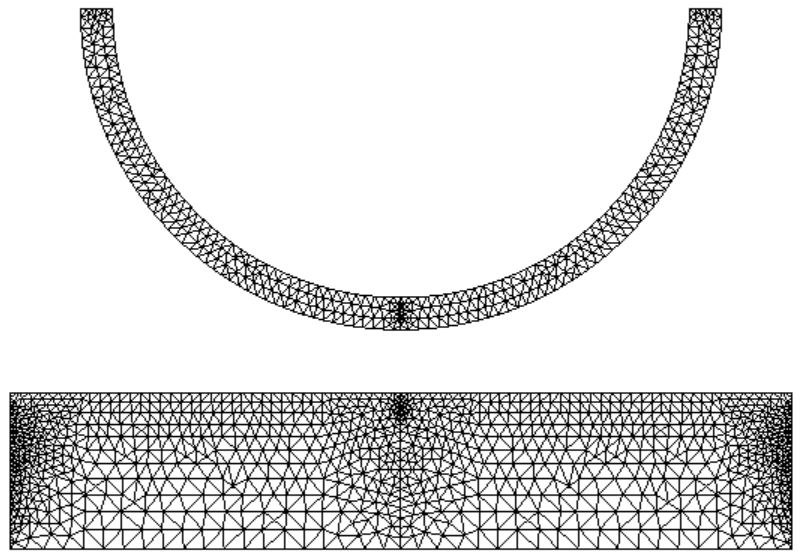
\includegraphics[width=0.4\textwidth]{./images/contact/ref_mesh.png}\quad
		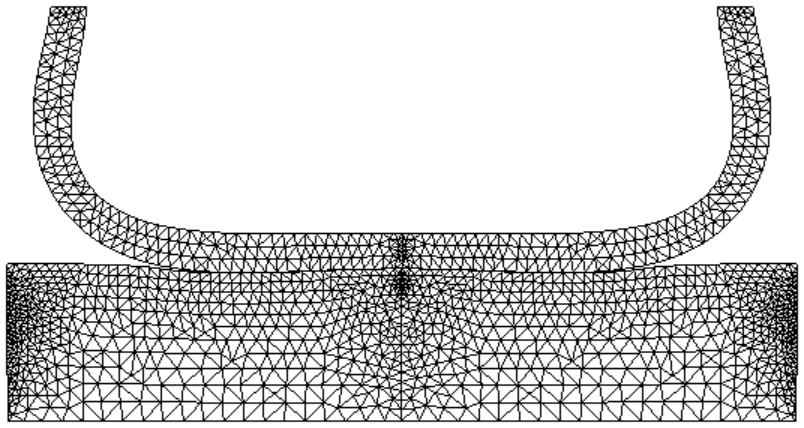
\includegraphics[width=0.4\textwidth]{./images/contact/def_mesh_1,1.png}
	\end{center}
\end{frame}

\begin{frame}\frametitle{Ring on block}
	Basis construction
	\begin{center}
		\hspace{-.7cm}
		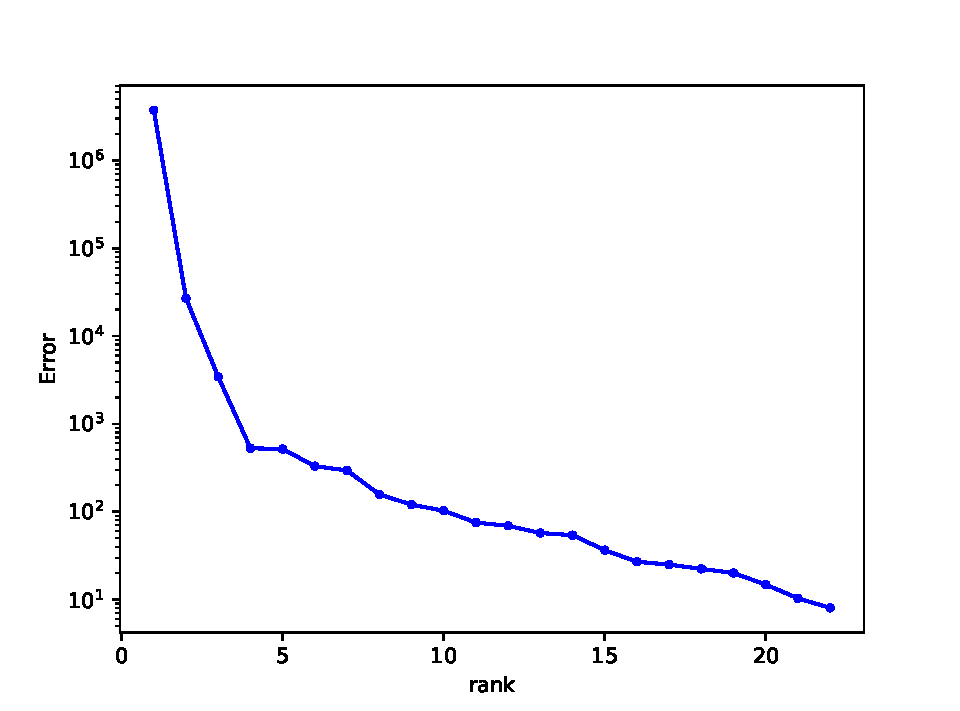
\includegraphics[width=.55\textwidth]{./images/contact/sgv_ring.pdf}
		\hspace{-.7cm}
		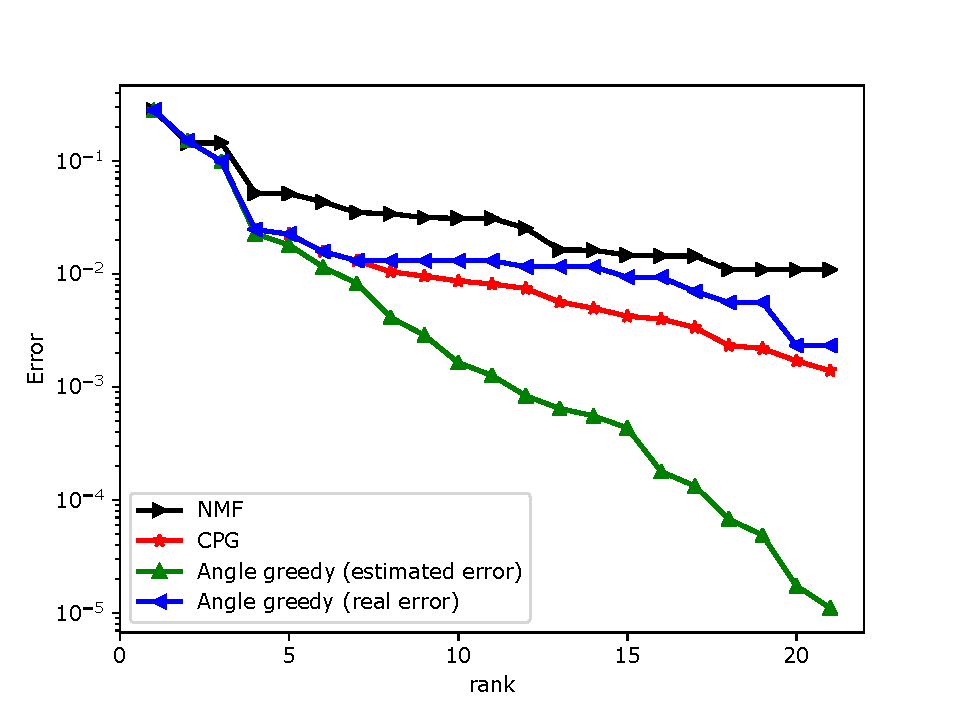
\includegraphics[width=.55\textwidth]{./images/contact/nmf_ring.pdf}
		\small{\hspace{1.8cm} \bl{Primal}basis
			\hspace{3.4cm} \ma{Dual}basis}
	\end{center}
\end{frame}


\appendix\begin{frame}
	\frametitle{Cone-projected greedy algorithm}
	\vspace{-0.4cm}
	\begin{algorithm}[H]
		\caption{Cone-projected weak greedy algorithm}
		\begin{algorithmic}[1]
			\Statex \textbf{\underline{Input :}}
			$\mathcal{P}^\mathrm{tr}$, $\widecheck\Gamma_1^{c}$
			and $\epsilon_{\rm du}>0$
			\State Compute $\mathcal S_{\rm du}
			= \{\widecheck\lambda(\mu;\cdot)\}_{\mu\in\mathcal{P}^\mathrm{tr}}$
			\State Set $\widecheck K_0 = \{ 0\}$, $n=1$ and $r_1 =
			{\mathrm{max}}_{\mu \in\mathcal P^{\mathrm{tr}}}\| \widecheck\lambda(\mu;\cdot)\|_{\ell^\infty(\widecheck \Gamma_1^{c})}$
			\While{($r_n >\epsilon_{\rm du}$)}
			\State Search  \bl{$\mu_n\in
				{\mathrm{argmax}}_{\mu \in\mathcal P^{\mathrm{tr}}}\ \| \widecheck\lambda(\mu;\cdot)-\Pi_{\gr{\widecheck K_{n-1}}}(\widecheck\lambda(\mu;\cdot))\|_{\ell^\infty(\widecheck{\Gamma}_{1}^{c,{\rm tr}})}$}
			\State Set $\gr{\widecheck K_n := {\rm span}_+\{\widecheck K_{n-1},\widecheck\lambda(\mu_{n};\cdot)\}}$
			\State Set $n=n+1$
			\State Set $r_{n} := 
			{\mathrm{max}}_{\mu \in\mathcal P^{\mathrm{tr}}}\ \| \widecheck\lambda(\mu;\cdot)-\Pi_{\widecheck K_{n-1}}(\widecheck\lambda(\mu;\cdot))\|_{\ell^\infty(\widecheck{\Gamma}_{1}^{c})}$\label{mx}
			\EndWhile
			\State Set $R:=n-1$
			\Statex \textbf{\underline {Output :}}
			$\widecheck W_R:=\widecheck K_{R}$
			\vspace{0.2cm}
		\end{algorithmic}
	\end{algorithm}
	\vspace{-0.3cm}
	$\rightarrow$ Python {cvxopt} library for positive projections
\end{frame}


 \end{document}


